\chapter{Giới thiệu}
\label{Chapter1}

Việc sử dụng mạng nơ-ron nhiều tầng ẩn trong các ứng dụng trí tuệ nhân tạo ngày càng chiếm một vị trí quan trọng khi mà các bài toán khó của học máy truyền thống trong việc xử lý ảnh và video, xử lý ngôn ngữ tự nhiên như: dịch máy tự động, nhận diện mặt người, phát hiện đồ vật,... đã phần nào được giải quyết và ngày càng được cải tiến.

Mạng nơ-ron nhiều tầng ẩn là một mạng nơ-ron nhân tạo gồm ba loại tầng chính: tầng nhập, các tầng ẩn, và tầng xuất. Việc có nhiều tầng ẩn cũng là một trong những lý do giúp cho mạng nơ-ron nhiều tầng ẩn có thể giải quyết các bài toán khó mà các thuật toán học máy truyền thống không giải quyết được. Mặc dù vẫn còn nhiều ý kiến về việc sử dụng nhiều tầng ẩn có thực sự cần thiết như công trình của Jimmy Lei Ba \cite{ba2013dodeepnets} chứng minh được rằng một mạng nơ-ron nông (shallow network) vẫn có thể xấp xỉ kết quả của một mạng nơ-ron nhiều tầng ẩn. Tuy nhiên, để đạt được kết quả đó, bài báo phải sử dụng một tập dữ liệu có kích thước rất lớn và vẫn phải huấn luyện một mạng nơ-ron nhiều tầng ẩn có độ chính xác khá cao. Ngoài việc mạng nơ-ron nhiều tầng ẩn có thể giúp cho quá trình thiết kế mô hình cho từng bài toán dễ dàng hơn \cite{nielsen2015neural} thì sức mạnh rút trích đặc trưng tự động cũng đã được chỉ ra trong nhiều bài báo khác: Yoshua Bengio và Yann Lecun lý giải rằng với nhiều tầng ẩn, mạng nơ-ron có thể ``học'' được từ đặc trưng đơn giản (low-level features) và tạo thành các đặc trưng phức tạp hơn (higher-level features) \cite{bengio2007scaling}; một công trình khác của Yoshua Bengio cho thấy sức mạnh của mạng nơ-ron nhiều tầng ẩn khi nó có thể giải quyết các bài toán mà các mạng nơ-ron ít tầng ẩn hơn không giải quyết được \cite{bengio2009learning}.

\begin{figure}[htp]
\centering
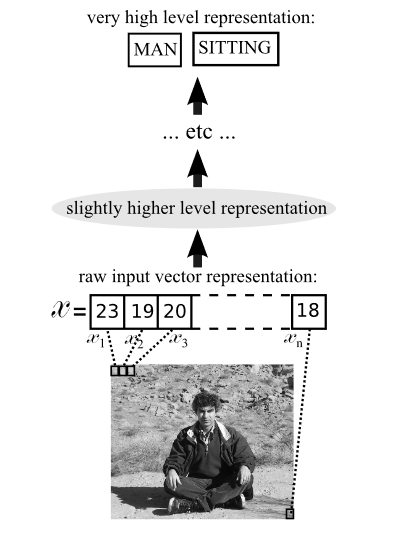
\includegraphics[width=65 mm]{images/layers-features.png}
\caption{Minh hoạ quá trình mạng nơ-ron ``học'' từ các đặc trưng đơn giản, như các điểm ảnh, tạo thành các đặc trưng phức tạp hơn, như câu mô tả. \cite{bengio2009learning}}
\label{fig:layers-features}
\end{figure}

Tuy nhiên, mạng nơ-ron có quá nhiều tầng ẩn sẽ khiến cho độ chính xác trong tập huấn luyện ngày càng tăng nhưng độ chính xác trong tập kiểm thử ngày càng giảm. Đây là biểu hiện của việc mô hình bị overfit, đồng nghĩa với việc mô hình chỉ ``ghi nhớ'' tập huấn luyện nhưng không thể tổng quát hóa những đặc trưng đã học để tiến hành đưa ra dự đoán trên tập kiểm thử. Ngược lại, nếu mạng nơ-ron quá đơn giản, có thể có ít tầng ẩn hoặc mỗi tầng ẩn có số lượng nơ-ron ít, thì mô hình đó không đủ khả năng để rút trích ra những đặc trưng có ý nghĩa mà mô hình có thể học khiến cho độ chính xác ở cả hai tập dữ liệu huấn luyện và kiểm thử đều giảm.

\begin{figure}[htp]
\centering
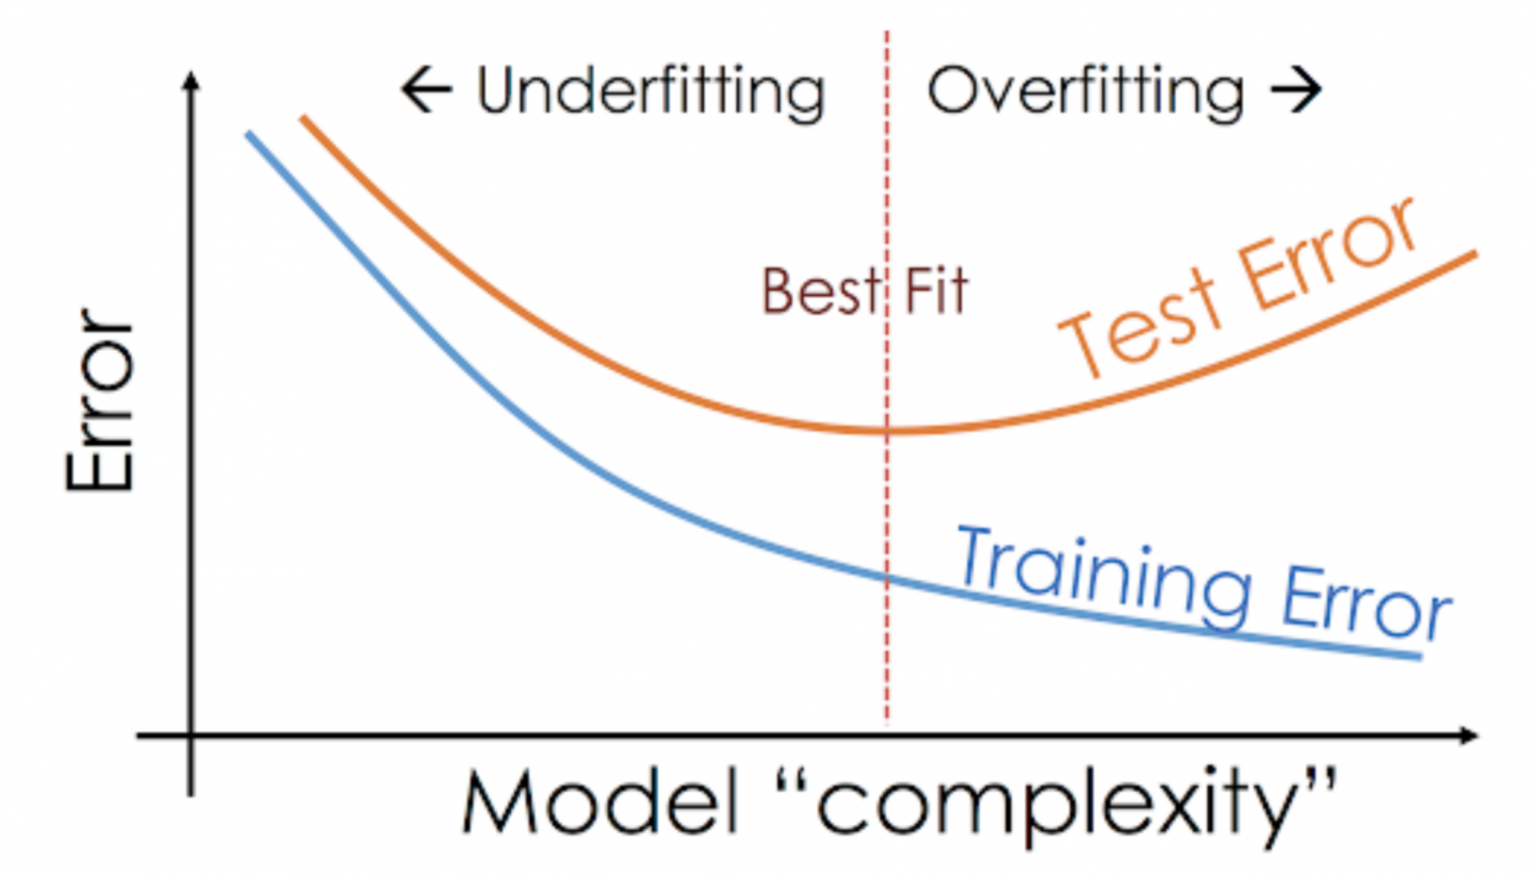
\includegraphics[width=100 mm]{images/under-over.png}
\caption{Minh họa cho mô hình overfit và underfit. \cite{underoverfit}}
\label{fig:under-over}
\end{figure}

Một mạng nơ-ron nhiều tầng ẩn được xem là tổng quát hoá tốt trên một bài toán khi sự sai khác giữa giá trị dự đoán của mạng nơ-ron và giá trị nhãn của dữ liệu ngoài tập huấn luyện là đủ nhỏ (trong bài toán huấn luyện có giám sát). Để đạt được kết quả đó, mạng nơ-ron nhiều tầng ẩn cần đi tìm một bộ trọng số phù hợp cho từng bài toán cụ thể. Việc đi tìm bộ trọng số này được thực hiện thông qua quá trình tối ưu hoá mạng nơ-ron nhiều tầng ẩn.

Bài toán tối ưu hoá mạng nơ-ron nhiều tầng ẩn nhận dữ liệu nhập là hàm chi phí nhận bộ trọng số của mạng nơ-ron nhiều tầng ẩn làm tham số. Hàm chi phí cho biết sự sai lệch giữa kết quả dự đoán của mạng nơ-ron so với giá trị đúng. Giá trị sai lệch này còn được gọi là độ lỗi. Sau quá trình tối ưu ta mong muốn có được một bộ trọng số của mạng nơ-ron nhiều tầng ẩn cho độ lỗi trong cả hai tập dữ liệu huấn luyện và tập dữ liệu kiểm tra là đủ nhỏ.

\begin{figure}[htp]
\centering
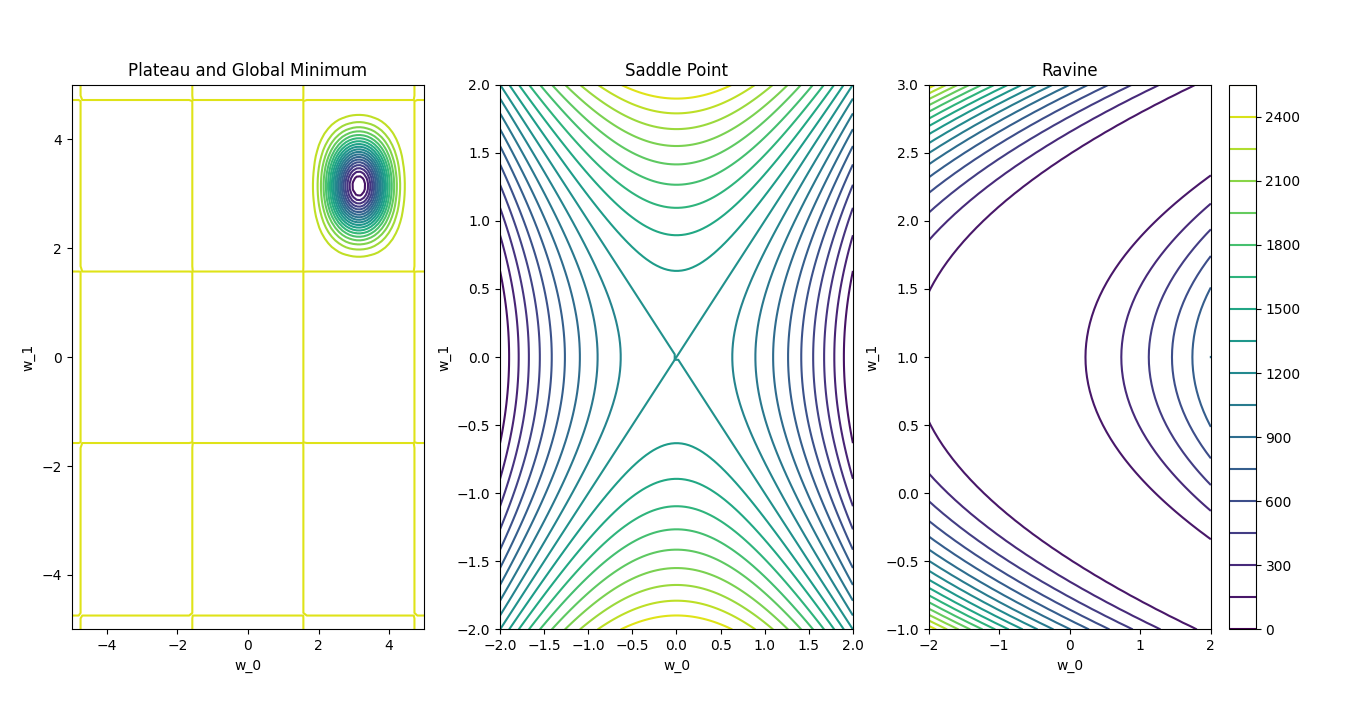
\includegraphics[width=120 mm]{images/cricial-point-contour.png}
\caption{Đồ thị contour cho những điểm critical point: vùng bằng phẳng có một cực tiểu (trái), điểm yên ngựa (giữa), vùng rãnh hẹp (phải).}
\label{fig:cricial-point-contour}
\end{figure}

Việc tối ưu hoá mạng nơ-ron có thể hiểu là quá trình đi tìm cực tiểu của hàm chi phí bằng cách thay đổi giá trị của bộ trọng số. Từ đó, ta cũng có thể hiểu quá trình tối ưu hoá mạng nơ-ron là quá trình di chuyển trong mặt phẳng lỗi để tìm được tọa độ của một điểm trên mặt phẳng được định nghĩa bởi hàm lỗi cho giá trị độ lỗi là đủ nhỏ. Tuy nhiên, việc di chuyển trong mặt phẳng lỗi gặp nhiều khó khăn. Li Hao và cộng sự \cite{li2018visualizing} cho thấy rằng sự hỗn loạn của mặt phẳng lỗi ngày càng tăng khi số tầng ẩn trọng mạng nơ-ron ngày càng tăng. Sự hỗn loạn này được cấu thành từ nhiều ``critical point'', những điểm có gradient bằng 0, như cực tiểu địa phương, điểm yên ngựa, hợp với các vùng bằng phẳng, và vùng rãnh hẹp.

\begin{figure}[htp]
\centering
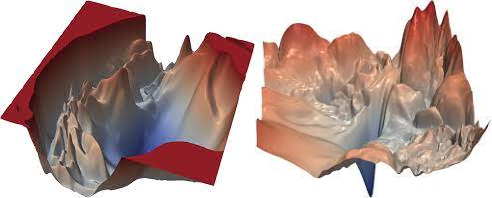
\includegraphics[width=120 mm]{images/resnet-loss.png}
\caption{Bề mặt lỗi của mô hình ResNet-110 (trái) và bề mặt lỗi của mô hình ResNet-56 (phải). \cite{li2018visualizing}}
\label{fig:resnet-loss}
\end{figure}

Các điểm cực tiểu địa phương từng được xem như là nguyên nhân chính gây ra sự khó khăn trong việc tối ưu hoá mạng nơ-ron có nhiều tầng ẩn, nhưng nghiên cứu của Quynh Nguyen và Matthias Hein \cite{nguyen2017thelosssurface} cũng như công trình của Anna Choromanska và cộng sự \cite{choromanska2014thelosssurface} đã chỉ ra rằng khi số lượng nơ-ron trong một tầng nhiều hơn điểm dữ liệu huấn luyện và các điểm dữ liệu độc lập tuyến tính với nhau thì hầu hết các điểm cực tiểu là cực tiểu toàn cục (hoặc có độ lỗi rất gần với cực tiểu toàn cục) và việc đi tìm cực tiểu toàn cục thật sự có thể mất nhiều thời gian nhưng cho hiệu quả không đáng kể. Vì thế cực tiểu địa phương không phải là nguyên nhân chính dẫn đến sự hội tụ chậm trong quá trình huấn luyện mà các điểm yên ngựa được bao bọc bởi vùng bằng phẳng mới là nguyên nhân chính dẫn đến những khó khăn trong việc tối ưu hoá mạng nơ-ron nhiều tầng ẩn. Yann N. Dauphin đã chỉ ra rằng số lượng điểm yên ngựa tăng lên theo tỷ lệ hàm mũ với số lượng tầng ẩn có trong mạng \cite{dauphin2014identifying}, khiến cho điểm yên ngựa là điểm xuất hiện nhiều nhất so với các critical point khác như cực tiểu cục bộ. Khi số lượng tầng ẩn quá lớn thì tất cả các điểm critical point sẽ là điểm yên ngựa và các điểm cực tiểu tìm được đều có độ lỗi ngang với cực tiểu toàn cục. Thêm nữa, các điểm yên ngựa thường được bao bọc bởi một vùng bằng phẳng, là vùng mà tại đó đạo hàm xấp xỉ gần bằng 0, làm chậm tốc độ của đa số các thuật toán tối ưu thường được sử dụng hiện nay. Vì thế, việc tránh và tìm được cách thoát ra khỏi điểm yên ngựa là quan trọng đối với các thuật toán tối ưu.

Trong thời gian đầu, việc huấn luyện mạng nơ-ron nhiều tầng ẩn sử dụng các phương pháp bậc nhất, các phương pháp này chỉ sử dụng đạo hàm bậc nhất của bề mặt lỗi tại vị trí hiện tại. Việc sử dụng đạo hàm bậc nhất/gradient sẽ cho biết hướng có độ dốc lớn nhất của bề mặt lỗi tại một điểm. Vì vậy, các phương pháp bậc nhất thường chỉ thực hiện những bước cập nhật rất nhỏ theo hướng gradient để tránh trường hợp bị vượt qua khỏi những vùng thấp hơn có khả năng chứa cực tiểu của bề mặt lỗi. Các phương pháp bậc nhất thường không gặp vấn đề mắc kẹt tại điểm yên ngựa vì hướng của gradient luôn đảm bảo tìm thấy một điểm mới có độ lỗi nhỏ hơn điểm hiện tại (nếu điểm hiện tại không phải là critical point), nhưng thường bị mắc kẹt tại các vùng bằng phẳng xung quanh điểm yên ngựa. Một số phương pháp áp dụng nguyên lý về quán tính để gia tăng tốc độ khi gặp những chiều di chuyển ổn định để nhanh chóng vượt qua vùng bằng phẳng.

\begin{figure}[htp]
\centering
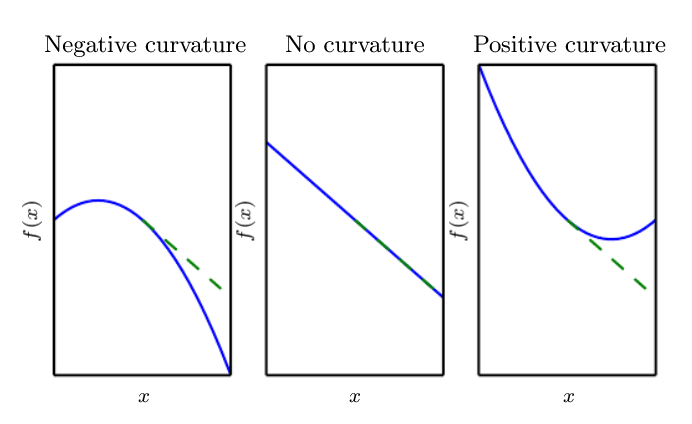
\includegraphics[width=120 mm]{images/hessian.png}
\caption{Mô tả điểm yếu của các thuật toán 1st-order không thể phân biệt đường cong xuống (trái), mặt phẳng (giữa), đường cong lên (phải). \cite{goodfellow2016deeplearning}}
\label{fig:hessian}
\end{figure}

Do đạo hàm bậc nhất thiếu đi thông tin về độ cong bề mặt lỗi, nên các thuật toán bậc nhất không thể tăng tốc tại các vùng có độ cong thấp (low-curvature) và giảm tốc khi gặp vùng có độ cong cao (high-curvature) như các thuật toán sử dụng đạo hàm bậc hai. Tuy nhiên, các phương pháp bậc hai, như thuật toán Newton, thường bị các điểm cực tiểu và cực đại ``thu hút'' nên dễ dàng bị mắc kẹt tại các điểm yên ngựa, tại đó vừa là cực tiểu trên chiều này nhưng là cực đại trên chiều khác. Để giải quyết hiện tượng này, một số cải tiến loại bỏ hoàn toàn chiều có độ cong hướng xuống tại điểm đang xét. Tuy nhiên, cách giải quyết này không đảm bảo chiều bị loại bỏ là chiều mà tại đó điểm yên ngựa là cực đại, dẫn đến hướng ra không được xem xét và thuật toán vẫn mắc kẹt tại điểm yên ngựa. Một cách cải tiến khác là sử dụng vùng tin cậy (trust region) bằng cách cộng thêm một hệ số dampening factor $\alpha$ vào công thức cập nhật. Hệ số này đảm bảo rằng ma trận Hessian là một ma trận xác định dương (positive definite), là ma trận mà tất cả phần tử trong ma trận đều không âm. Cách cải tiến này tuy có thể giúp thuật toán thoát khỏi vùng yên ngựa nhưng lại có thể mất nhiều thời gian để thoát khỏi vùng bằng phẳng nếu hệ số $\alpha$ quá lớn. Mặt khác, việc tính toán đạo hàm bậc hai đòi hỏi nhiều chi phí tính toán và tiêu tốn bộ nhớ cấp số mũ với số lượng trọng số của mạng. Đối với các mạng nơ-ron nhiều tầng ẩn mà số lượng trọng số có thể lên đến hàng tỷ thì đây là bất khả thi. Vì vậy, một số phương pháp bậc nhất thực hiện xấp xỉ thông tin của đạo hàm bậc hai (cụ thể là xấp xỉ ma trận Hessian) từ gradient để thực hiện cập nhật bước nhảy tối ưu hơn cho từng trọng số. Họ các thuật toán này được gọi là các thuật toán có tỉ lệ học thích ứng (adaptive learning rate).

Nhìn chung, mỗi nhóm phương pháp cố gắng khắc phục một vấn đề của bài toán, nhưng lại không hoạt động tốt trong những trường hợp mà nhóm phương pháp còn lại có thể giải quyết được. Cụ thể là với những phương pháp sử dụng gradient kết hợp với một số phương pháp tăng tốc, việc cập nhật chỉ được thực hiện theo hướng của gradient mà không có nhiều thông tin về chiều dài mà bước cập nhật nên thực hiện, cũng như hướng của gradient không phải lúc nào cũng là hướng đi tốt nhất.

\begin{figure}[htp]
\centering
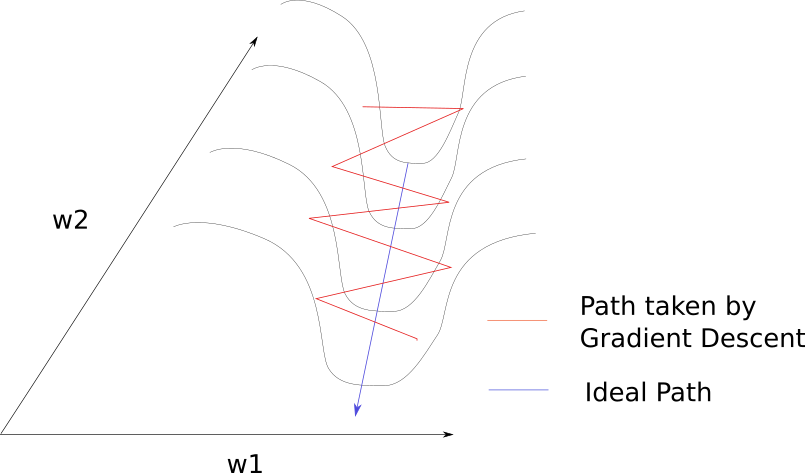
\includegraphics[width=100 mm]{images/valley.png}
\caption{Minh họa cho hướng đi của gradient trong trường hợp di chuyển trong rãnh hẹp. \cite{gradientvalley}}
\label{fig:valley}
\end{figure}

Một trường hợp thể hiện hướng đi của gradient không phù hợp là trường hợp di chuyển trong rãnh hẹp, hai bên có độ dốc cao và một rãnh thấp ở giữa. Khi đó, gradient sẽ hướng về phía sườn dốc còn lại thay vì hướng theo rãnh thấp, khiến cho điểm di chuyển bị dao động mạnh trong khi độ lỗi không giảm nhiều. Hiện tượng dao động này có thể được khắc phục một phần bằng quán tính, tuy nhiên chính quán tính lại có thể tạo ra một số vấn đề như đi vượt khỏi điểm cực tiểu mong muốn. Trong khi đó, những phương pháp sử dụng tỉ lệ học thích ứng mặc dù di chuyển tốt hơn về phía điểm cực tiểu, nhưng lại thực hiện những bước cập nhật rất chậm. Ngoài ra, lợi thế của tỉ lệ học riêng biệt cho từng trọng số cũng bị suy giảm nếu như các trọng số phụ thuộc vào nhau.

Lấy ý tưởng từ những phương pháp trên, Diederik P. Kingma và Jimmy Lei Ba đã đề xuất một thuật toán tối ưu bậc nhất cho mạng nơ-ron nhiều tầng ẩn với tốc độ cao hơn so với hầu hết những thuật toán trước đó \cite{kingma2014adam}. Công trình này, \emph{``Adam, A Method for Stochastic Optimization''}, được công bố tại hội nghị \emph{``International Conference on Learning Representation 2015''}. Ý tưởng của thuật toán là kết hợp hai hướng tiếp cận trước đó: (1) sử dụng quán tính để tăng tốc và giảm dao động, và (2) thích ứng lượng cập nhật cho từng trọng số. Nhờ sự kết hợp này, Adam kế thừa được nhiều ưu điểm, đồng thời khắc phục những hạn chế của các hướng tiếp cận trên khi có thể tăng giảm độ dài bước cập nhật tùy theo điều kiện bề mặt lỗi, cũng như điều chỉnh tỉ lệ học thích ứng cho từng trọng số của mạng nơ-ron. Trong khóa luận này, chúng tôi tìm hiểu và cài đặt lại thuật toán Adam cùng với các thuật toán liên quan. Chúng tôi cũng thực hiện thêm các thí nghiệm nhằm phân tích và làm rõ cách mỗi phương pháp giải quyết các khó khăn trong việc huấn luyện mạng nơ-ron nhiều tầng ẩn. Ngoài ra, chúng tôi cũng sử dụng tính toán song song trên GPU để tăng tốc độ xử lí cho các thí nghiệm.

Phần còn lại của khóa luận được trình bày như sau:

\begin{itemize}
	\item Chương 2 giới thiệu sơ lược về mạng nơ-ron nhiều tầng ẩn và quá trình huấn luyện, cũng như nguyên lý của thuật toán Gradient Descent.
	\item Chương 3 trình bày về thuật toán Adam và các thuật toán nền tảng. Chương này là phần chính của khóa luận.
	\item Chương 4 trình bày về các thí nghiệm về nguyên lý cũng như thực tiễn để phân tích các tính chất của thuật toán Adam.
	\item Cuối cùng, chương 5 trình bày kết luận và hướng phát triển.
\end{itemize}
